\documentclass[preprint]{style}
\pagenumbering{arabic}

\usepackage{paralist}
\usepackage{graphicx}
\usepackage{url}
\usepackage{amsmath}



% This gets rid of the block of whitespace on the first page
\makeatletter
\let\@copyrightspace\relax
\makeatother


\addtolength{\topmargin}{-.07in}
\addtolength{\textheight}{.07in}

%\addtolength{\oddsidemargin}{-0.08in}
%\addtolength{\evensidemargin}{-0.08in}
%\addtolength{\textwidth}{0.08in}



\begin{document}

\title{Medical Concept Extraction}

\numberofauthors{3}
\author{
\alignauthor
Tristan Naumann\\
\affaddr{MIT EECS}
\email{tjn@mit.edu}
\alignauthor
Samantha Ainsley\\
\affaddr{MIT EECS}
\email{ainsley@mit.edu}
\alignauthor
Salman Ahmad\\
\affaddr{MIT EECS}
\email{saahmad@mit.edu}
}

\date{14 December 2012}

\maketitle
\begin{abstract}

This paper presents a system for extracting medical concepts from patient hospital records. Hospitals and medical practices are increasingly switching to electronic medical records--this trend has opened the doors to exciting applications for Natural Language Processing in medicine and biology. One such application is concept extraction: identifying high-level semantic labels in a body of text. Concept extraction on medical records is useful in automating analysis tasks that would otherwise have to be done manually. For example, hospital administrators may want to tabulate what medications are being prescribed the most. Insurance companies may want to ensure that patients receive proper care and are billed accordingly for fraud detection and auditing purposes. Government agencies may be interested in exploring and better understanding public health trends. Automatic concept extraction systems help to streamline such critical yet laborious tasks.

In service of that end, we present an algorithm and system that is capable of classifying words in medical records across four different medically-relevant categories: (1) problems, (2) tests, (3) treatments, and (4) non-medical terms. This is useful not only in granting end users the ability to analyze medical records, but also in supporting other higher-level Natural Language Processing and learning systems. This paper describes the system's design, implementation, and performance when tested on set of 500 pre-annotated medical records from Boston-area hospitals.


\end{abstract}

\section{Introduction}

Lorem ipsum dolor sit amet, consectetur adipisicing elit, sed do eiusmod tempor incididunt ut labore et dolore magna aliqua. Ut enim ad minim veniam, quis nostrud exercitation ullamco laboris nisi ut aliquip ex ea commodo consequat. Duis aute irure dolor in reprehenderit in voluptate velit esse cillum dolore eu fugiat nulla pariatur. Excepteur sint occaecat cupidatat non proident, sunt in culpa qui officia deserunt mollit anim id est laborum.

\section{Related Work}

\section{Machine Learning}

Talk about multi-class classification

\subsection{Support Vector Machines}

\subsection{Linear Regression}

\subsection{Conditional Random Fields}

\section{Challenges}

\subsection{High Dimensionality}

\subsection{Biased Data}

\subsection{Amount of Data}

Low amounts of train data with high amounts of tests data.

\subsection{Data Usage Agreements}

\section{Design}

\subsection{Data Flow \& Classification Task}
Our system considers each document to be a stream of words grouped by sentences, and it attempts to provide the correct concept classification for each word. In order to identify the appropriate concept, our system considers natural language features for each document in successively broader contexts. Specifically, we first consider features using only the word itself as context, next we consider features which span the sentence, and last we consider n-gram features. In the sections that follow we discuss the linguistic features used in each context.

\subsection{Word Features}
Using only the word as context we are able to generate several interesting linguistic features. These features generally take on one of three forms: (1) intrinsic property of the word, (2) binary indicator for properties that we think are interesting, and (3) various techniques that map words into a small dimensional space such as stemming and word shape.

\subsubsection{Word}
The most obvious property of each word is perhaps the word itself. Since there is no linguistically meaningful, strict ordering over words, each word is represented as its own dimension. Consequently adding a baseline feature containing the word increases the dimension of our feature space to the size of the vocabulary in the training data.

\subsubsection{Length}
The next most obvious property of each word is its length. Unlike using the word as a feature, there is a strict ordering over length and consequently the addition of this feature increases the dimension of the space by only $1$. While the linguistic merit of length as a feature can be debated in conventional natural language processing, we felt it would play a large role in medical language in order to distinguish treatments, tests, and problems from words without a concept. Intuitively this is because often times treatments in the form of medications consist of long medical names, as do some of the words in medically described problems and tests.

\subsubsection{MIT Regular Expressions}
In order to capture some general characteristics of each word we included a set of regular expressions each of which adds a dimension to our classification. The characteristics we chose are as follows:
\begin{itemize}
\item {\tt INITCAP}: first letter is capitalized and alphabetic,
\item {\tt ALLCAPS}: entire word is capitalized and alphabetic,
\item {\tt CAPSMIX}: the word is a mix of capital and lowercase alphabetic characters,
\item {\tt HASDIGIT}: there is a digit in the word,
\item {\tt SINGLEDIGIT}: the token is a single digit,
\item {\tt DOUBLEDIGIT}: the token is a two digits,
\item {\tt FOURDIGITS}: the token is a series of four digits,
\item {\tt NATURALNUM}: the token is a natural number,
\item {\tt REALNUM}: the token is a real number,
\item {\tt ALPHANUM}: the token contains only digits and alphabetic characters,
\item {\tt HASDASH}: the token has a dash,
\item {\tt PUNCTUATION}: the token is punctuation,
\item {\tt PHONE1}: the token is a phone number,
\item {\tt PHONE2}: the token is a phone number with area code,
\item {\tt FIVEDIGIT}: the token is a series of five digits,
\item {\tt NOVOWELS}: the token does not contain vowels (i.e. abbreviations),
\item {\tt HASDASHNUMALPHA}: the token consists of a dash, numbers, and alphabetic characters, 
\item {\tt DATESEPERATOR}: the token is a date separator (e.g. {\tt [-/]})
\end{itemize}


\subsubsection{Porter Stemmer}
Our CRF F1 scores went from 0.58 to 0.82

\subsubsection{Lancaster Stemmer}

\subsubsection{Snowball Stemmer}

\subsubsection{Word Shape}

\subsection{Sentence Features}

\subsubsection{Part of Speech}

\subsubsection{WordNet Lemmatizer}

\subsubsection{Formatted Text}

\subsection{N-gram Features}

\subsubsection{Previous}

\subsubsection{Next}

\subsection{Parameter Tuning}

\begin{figure}
\begin{center}
	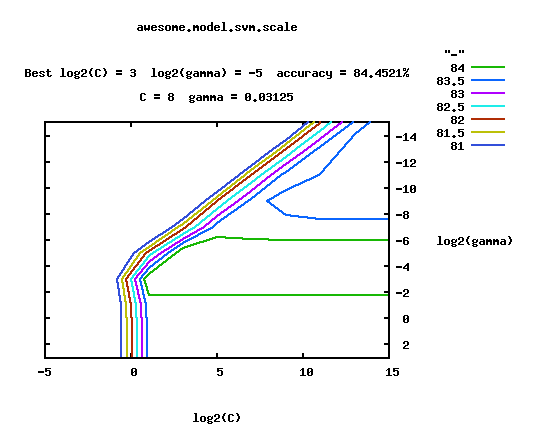
\includegraphics[width=1\columnwidth]{figures/parameter-selection.png}
\end{center}
\caption{An illustration of the grid search process to identify the best parameters values for training the SVM model.}
\label{fig:parameter_selection}
\end{figure}

\begin{itemize}

\item Grid search and grid search image

\item Include that PNG image from easy.py

\item Cross validation

\end{itemize}




\section{System}

\subsection{Code Architecture}

\begin{figure}
\begin{center}
	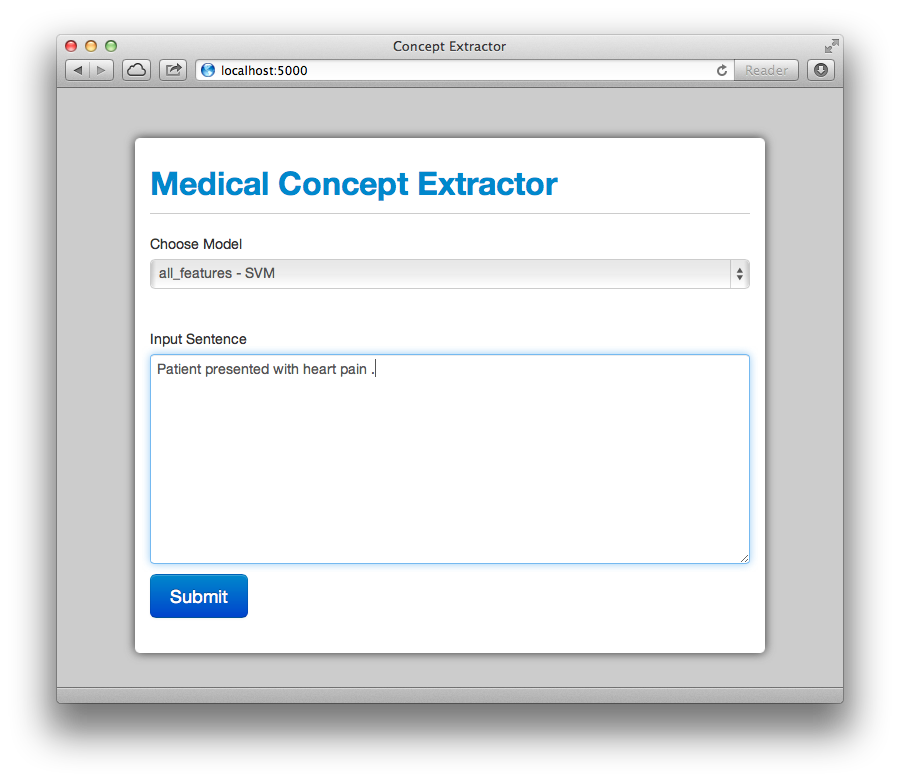
\includegraphics[width=1\columnwidth]{figures/system.png}
\end{center}
\caption{An overview of the system and codebase.}
\label{fig:system}
\end{figure}


We built a fairly comprehensive framework for applying machine learning techniques to NLP domains. We built out a series of useful and reusable library modules and command line utilities to perform various tasks. An overview of the codebase can be seen in Figure~\ref{fig:system} and  all of the code is available online at the following url:

{\tt https://github.com/tnaumann/ConceptExtraction}.

\subsubsection{Data Formats and File I/O}

\subsubsection{Feature Computation}

\subsubsection{Model Encapsulation and Serialization}

\subsubsection{Learning Algorithms}

\subsubsection{Data Organization and Directory Structure}

\subsubsection{Command-line Utilities}

\subsection{Web Service}

In addition to the various command line utilizes described in the previous section our system also includes a Web-based service that allows users to manually input a single sentence, select a model to use for prediction, and see the predicted labels that model generated for the input. Figure~\ref{fig:web_interface} shows a screenshot of the Web interface in use.

The Web service was written in Python and directly interoperates with the rest of the code base. To run the Web applications simply execute the {\tt web.py} file in the source tree. The Web app assumes that models have already been trained and placed into ``models'' directory in the source tree. By default, the application will host itself on port 5000. You can also see a live version of the Web service at:

{\tt http://saahmad.media.mit.edu:5000/ }

\begin{figure}
\begin{center}
	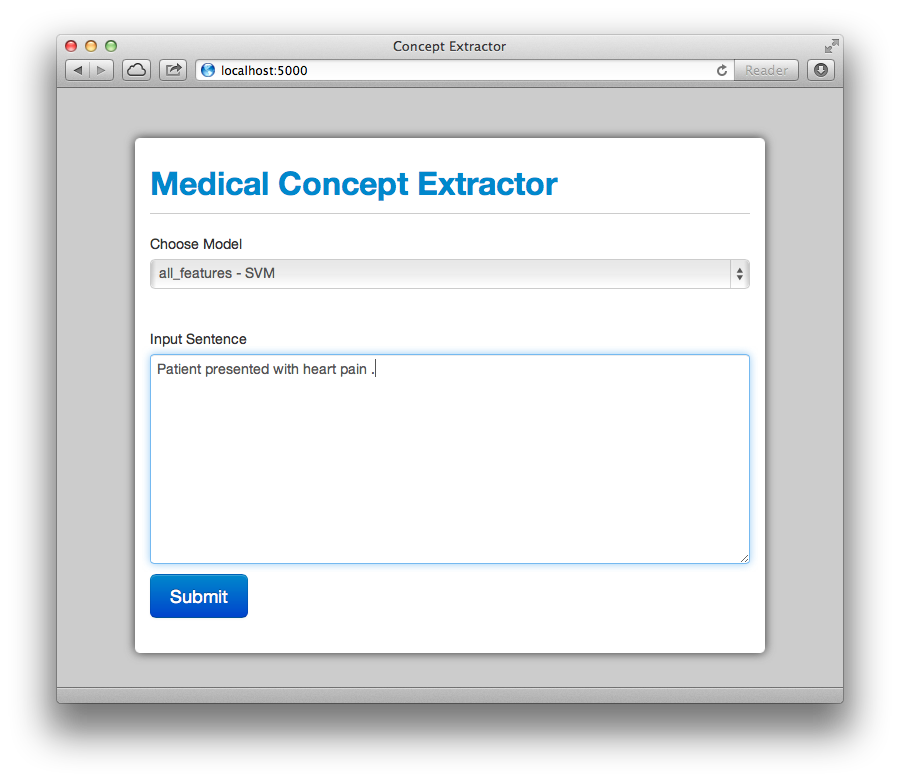
\includegraphics[width=1\columnwidth]{figures/web-interface.png}
\end{center}
\caption{The Web application interface that allows users to manually input a sentence and have it labeled using one of the previously-trained models. In this case we are using an SVM model that was trained using all of the features.}
\label{fig:web_interface}
\end{figure}


\subsection{Libraries}

Our code leveraged various 3rd party libraries for training the models and generating features. A summary of the libraries that we used is shown in the list below:

\begin{itemize}

\item {\tt libsvm} \cite{libsvm}: libsvm provides a fast implementation of Support Vector Machines. It includes a command line utility that takes a training data (with all of the features formatted in a sparse matrix representation) as input and outputs a SVM model trained on that data. It also includes a command line utility that allows users to specify a desired model and predict the classes on new input. Our code base forks process calls to these utilities to train SVM models, although a lot of the parameter tuning and feature selection is handled elsewhere in our codebase.

\item {\tt liblinear} \cite{liblinear}: lib linear is a linear classifier library that has special support multi-class classification. It also provides easy to use training and predicting command line utilities that accept a similar input format as libsvm.

\item {\tt crfsuite} \cite{crfsuite}: crfsuite is an implementation for conditional random fields and includes command line front ends to train a model on data and to predict the labels on an unseen data set. The data format for the input training files is also a sparse matrix representation but is slightly different from the format used by libsvm and lib linear. Our codebase nicely abstracts out these format differences and produces the right format depending on the model in use.

\item {\tt nltk} \cite{nltk}: nltk is a very popular NLP library written in Python. We leverage nltk to generate some of the features on our data. In particular, we utilize nltk's maximum-entropy part-of-speech tagging as well as many of its stemming algorithms.

\item {\tt flask} \cite{flask}: Flask is a micro Web framework written in Python. It contains a small yet useful set of features that allow developers to easily setup RESTful Web backends and an elegant tempting system to gracefully generate HTML. Flask is used to build the Web service portion of the project.

\end{itemize}
	

\section{Results}

\subsection{Data Set}

Talk about the competition and where the data came from. How large the data size is, how much we trained on, etc.

\subsection{Trained Models}

Describe the different feature-subsets that we trained and why.

\subsection{Runtime Performance}

How long each model took to train and how fast we can predict. Also discussion the hardware that was used to train and predict in terms of CPU speed, memory, etc.

\subsection{Classification Performance}

A table of a bunch of awesome results. We should present results by model type (SVM, CRF, LIN) and feature set.

\section{Discussion}

Talk about what we saw in terms of which was the best feature set and model. 

Be sure to include examples of cool cases where it caught a difficult label

Be sure to include FAILURE cases

\section{Conclusion and Future Work}

\subsection{Dimension Collapse}

\subsection{Feature Selection}

\subsection{Parameter Selection}

\subsection{More Data}


\section{Acknowledgments}

We sincerely thank Dr. Robert Berwick  and Geza Kovacs
for their guidance, help, and support.


%%%% May the Flow (Max-Flow, that is) be with you all.

%
% The following two commands are all you need in the
% initial runs of your .tex file to
% produce the bibliography for the citations in your paper.
\bibliographystyle{abbrv}
\bibliography{citations}  % sigproc.bib is the name of the Bibliography in this case

\balancecolumns
% That's all folks!
\end{document}
